\documentclass[12pt]{article}

\usepackage{amsmath, amsfonts, amssymb, amsthm, bbm, mathtools}
\usepackage{booktabs, fancyhdr, verbatim, graphicx, float, url}
\usepackage{algorithm}
\usepackage{algpseudocode}
\newenvironment{claim}[1]{\par\noindent\underline{Claim:}\space#1}{}
\newenvironment{claimproof}[1]{\par\noindent\underline{Proof:}\space#1}{\hfill $\blacksquare$}

\title{Final Project Report: QR Factorization on GPUs}
\author{Ryan Synk}

\begin{document}

\maketitle

\section*{Introduction}

This report outlines my work on implementing a fast QR factorization algorithm on a Graphics
Processing Unit (GPU). It closely follows a 2009 paper of Kerr et. al 
\cite{10.1145/1513895.1513904} and focuses on writing code to mimic the results found
in the paper.

\subsection*{Graphics Processing Units}

Graphics processing units (GPUs) are parallel processors initially designed for computing shaders
in computer graphics applications. In a Central Processing Unit (CPU), one large, powerful chip 
performs the computations. GPUs, on the other hand, consist of many small processing units, 
each capable of performing computations in parallel with one another. These small processing
units are referred to by NVIDIA, a GPU manufacturer, as Streaming Multiprocessors (SMs). 
Associated with each SM is a store of L1 cache memory. Each SM, in turn, can access a global 
L2 memory cache --- see figure \ref{fig:gpudiagram} for a diagram of a recent GPU. This 
architecture, with its combination of parallel processors and memory hierarchy, lends 
itself well to fine-grained parallelization --- and in the case of computer graphics, dense 
linear algebra calculations.

\begin{figure}[H]
    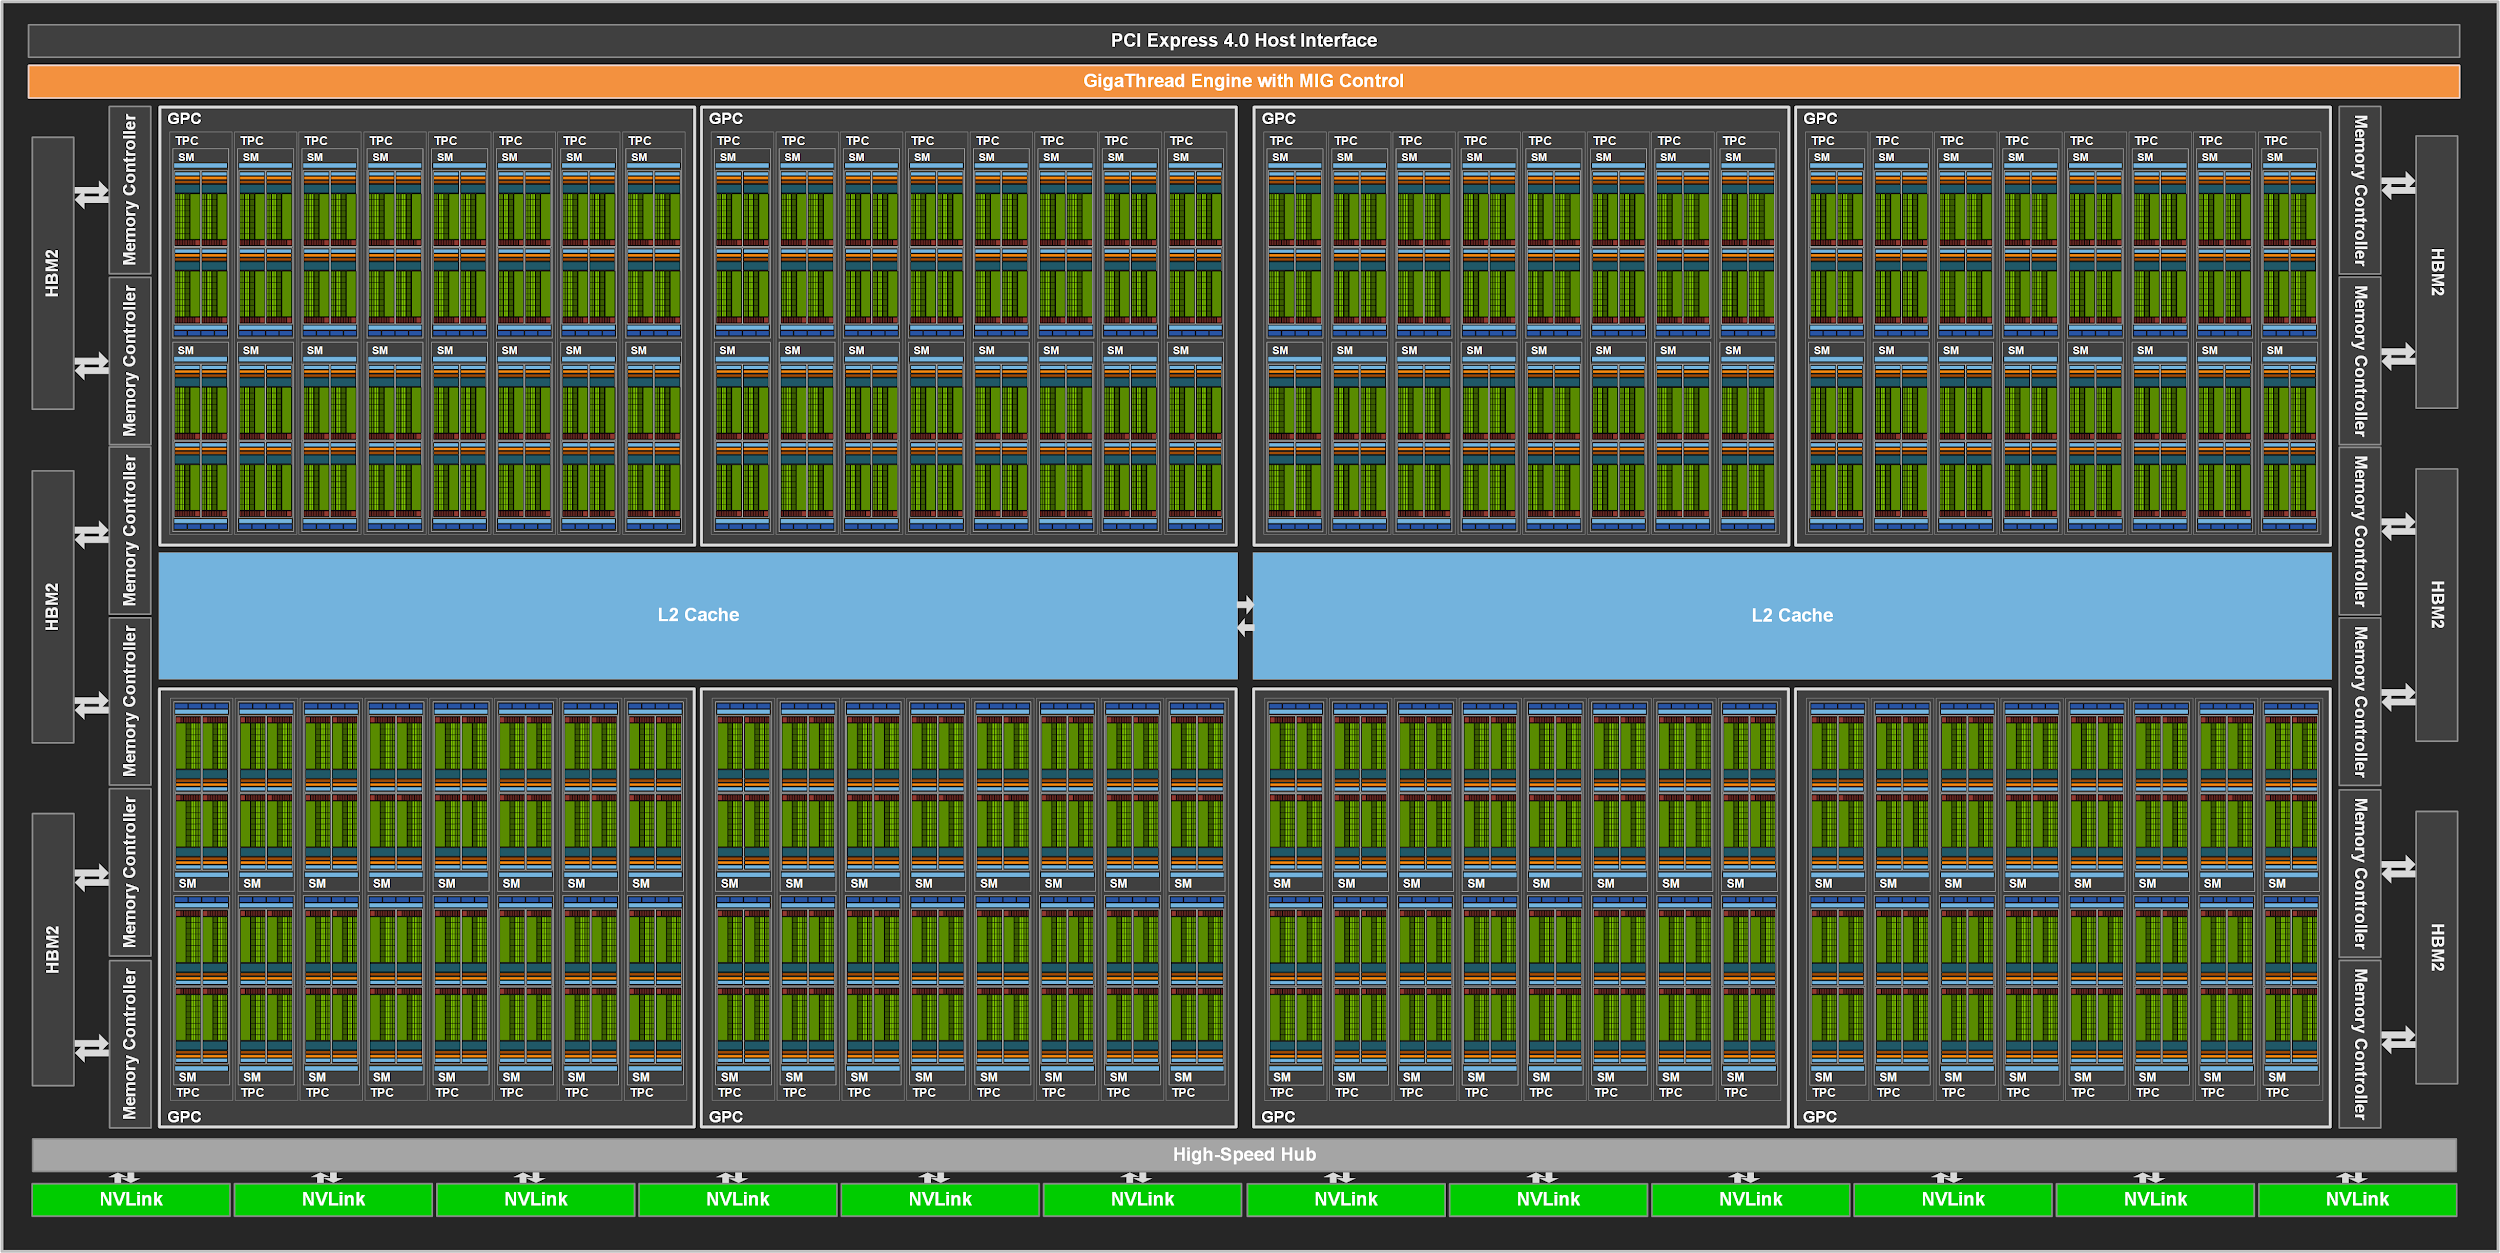
\includegraphics[scale=0.20]{gpu_diagram}
    \caption{NVIDIA Volta GPU. Source: \cite{volta_blogpost}}
    \label{fig:gpudiagram}
\end{figure}

Shortly after the advent of modern graphics processing units with programmable shaders, 
studies in the use of GPUs for scientific computing problems were conducted. In 2001, 
researchers implemented the first matrix-matrix multiplication algorithm for a GPU 
\cite{10.1145/582034.582089}. Eventually, certain applications running on GPUs began to 
outperform their counterparts on CPUs. In a 2005 paper (whose authors include UMD 
Professor Dinesh Manocha), a GPU implementation of LU factorization with partial 
pivoting was shown to outperform a CPU. \cite{1559955}. Scientific computing wasn't the only
field impacted by GPUs.

The training of deep neural networks is a process which involves large amounts of dense
matrix-vector and matrix-matrix multiplications. The discovery that GPUs are well-suited 
to accelerate this traning process was instrumental in the revolution of deep learning 
in the 2010s, helping to turn neural networks from theoretical curiosities into the 
ubiquitous and powerful models they are today.

Work still continues as researchers in numerical linear algebra and high-performance 
computing try to find ways that GPUs can accelerate their algorithms. High-performance 
computing systems are being built with more and more GPU accelerators in them, 
and the DOE's newest exascale supercomputer, Frontier, will be built with four times 
as many GPUs as CPUs \cite{frontier}.

\subsection*{QR Factorization}

In this report, we will develop a GPU-based method to solve the problem of factorizing 
an $m \times n$ matrix $A$ as the product $A = QR$. Here, $Q \in \mathbb{R}^{m \times m}$ 
is an $m \times m$ unitary matrix, and $R$ is an upper-triangular matrix. A number of basic
algorithms for finding such a decomposition exist, and they all follow the pattern of
successively zeroing out entries of $A$ below the main diagonal using unitary transformations.
These methods include

\begin{enumerate}
    \item Givens rotation factorization
    \item Gram-schmidt factorization
    \item Householder QR factorization
\end{enumerate}

For the latter, a series of Householder transformations are used to zero out entries 
below the diagonal of $A$. Given a vector $x \in \mathbb{R}^{n}$, a Householder matrix $P_x$ 
can be generated such that $P_x x = \|x\|e_1$ --- in other words, the matrix transforms
the vector $x$ into a multiple of the $1^{st}$ basis vector in $\mathbb{R}^{n}$.

The transformation $P_x$ is of the form
\begin{flalign*}
    P_x &= I - \frac{2}{v^{T}v}v v^{T} \\
    v &= x - \|x\|e_1
\end{flalign*}

If we choose $x_k$ to be the the vector in $\mathbb{R}^{n - k}$ consisting of entries of the
$k^{th}$ column of $A$, starting at the diagonal and moving downwards ($A(m:k, n)$ in 
MATLAB notation) we can create a householder transformation $P_k$ which zeros out the 
entries below the diagonal of the  $k^{th}$ column of $A$. See figure \ref{fig:householder_qr}
for a diagram.

\begin{figure}[H]
    \centering
    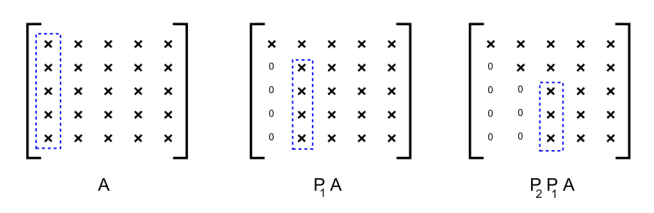
\includegraphics[scale=0.5]{qr_diagram}
    \caption{Successive householder transformations acting on $A$ Source: \cite{10.1145/1513895.1513904}}
    \label{fig:householder_qr}
\end{figure}

Importantly, the $P$ matrices don't need to be fully formed. If we define $\beta_k = \frac{2}{v_k^{T}v_k}$, then
\begin{flalign*}
    PA &= (I - \beta_k v_k v_k^{T}) A \\
    &= A - \beta_k v_k (A^{T} v_k)
\end{flalign*}

So we can perform a rank-one update to $A$ at each iteration. We can string these updates
together, and, since each of the $P_k$ transformations are unitary, we preserve the original
matrix:
\[
    A = (P_1^{T}P_2^{T}\dots P_k^{T})(P_k \dots P_2 P_1)A
\] 

And our QR decomposition is 
\begin{flalign*}
    Q &= (P_1^{T} P_2^{T}\dots P_{n-1}^{T}) \\
    R &= (P_{n-1} \dots P_2 P_1 A)
\end{flalign*}

So at each iteration, we make the following updates:
\begin{flalign*}
    R &\leftarrow (I - \beta_k v_k v_k^{T}) R \\
    Q &\leftarrow Q(I - \beta_K v_k v_k^{T})
\end{flalign*}

Putting this together gives the following $QR$ algorithm:

\begin{algorithm}
\caption{QR Factorization Via Householder}\label{alg:cap}
\begin{algorithmic}
\State Given $A\in\mathbb{R}^{mxn}$
\State $Q \gets I_m$ 
\State $R \gets A$
    \For{$k = 1:n$}
    \State $[v, \beta] = \mathbf{house}(R[k:m, 1:n])$ 
    \State $R[k:m, 1:n] = R[k:m, 1:n] - \beta v v^{T} R[k:m, 1:n]$
    \State $Q[1:m, k:m] = Q[1:m, k:m] - \beta Q[1:m, k:m]v v^{T}$
    \EndFor
\end{algorithmic}
\end{algorithm}

This $QR$ algorithm works well, but for our purposes it will require some modification
to run quickly on a GPU.

\section*{Algorithm}
As was mentioned before, GPUs can offer speedups to many different problems. However,
given the physical distance between host memory and the GPU, there is a nontrivial cost
in moving data from the CPU to the GPU. In many problems, the data in question is 
small enough to fit onto CPU cache, and thus can be done in the time it takes to 
move the data onto the GPU itself. Care must be taken in writing GPU code to make sure
that, when possible, all data that is moved onto the GPU stays on the GPU for the duration
of the the computation. And, before writing any code, the size of the problem in 
question should be examined to ensure that a GPU will offer an increased effiency.
In this way, GPUs will offer much greater speedups in computing $QR$ factorizations 
for \textbf{large} matrices, and our algorithm is tailored around that idea.

Additionally, when data is on the GPU, in order to maximize efficiency, as many computations
as possible should be performed in parallel. In this way,... As \cite{10.1145/1513895.1513904}
states, in the above algorithm, "the amount of computation per memory element fetched 
from global memory is quite low." Currently, the algorithm... So if we want to take advantage
of the speedups that a GPU has to offer, we will have to give the GPU a sufficient amount of 
work to do. In this way, we'd like to transition our computation from operating solely in
terms of matrix-vector products, and shift it to focusing on matrix-matrix products.

It is with this in mind that we turn to a 1985 result of Bischof and Van Loan
\cite{osti_6535818}. They showed that applying a series of rank-1 updates
\begin{flalign*}
    P &= P_1 P_2 \dots P_r \\
      &= (I - \beta_1 v_1 v_1^{T}) \dots (I - \beta_r v_r v_r^{T})
\end{flalign*}
Is equivalent to applying a rank-r update of the following form:
\begin{flalign*}
    P_{wy} &= P_1 P_2 \dots P_r \\
           &= I + YW^{T}
\end{flalign*}
For $m\times r$ matrices $W$ and $Y$, which are constructed from the vectors and scalars
$(\beta_i, v_i)$. Their construction is outlined in the following algorithm:

\begin{algorithm}
\caption{Construction of $W$, $Y$ matrices}\label{alg:wy}
\begin{algorithmic}
\State Given $v_1 \in \mathbb{R}^{n}, v_2 \in \mathbb{R}^{n-1} \dots v_r \in \mathbb{R}^{n - r + 1}$
\State Given $\beta_1, \dots \beta_r \in \mathbb{R}$
\State $Y = v_1$
\State $W = -\beta_1 * v_1$
    \For{$j = 2:r$}
    \State $z = -\beta_j v_j - \beta_j WY^{T} v_j$
    \State $W = [W z]$
    \State $Y = [Y v]$
    \EndFor
\end{algorithmic}
\end{algorithm}

So, given some set of $r$ Householder updates, we can generate matrices $W$ and $Y$ to
update the rest of our matrix with. This motivates Kerr et. al's Block Householder algorithm.
We first partition our matrix $A$ into block matrices of size $m \times r$:
\[
    A = \begin{pmatrix} 
            A_1 & A_2 & \dots & A_{\frac{n}{r}} 
        \end{pmatrix}
\] 

For a given block $A_k$, we compute the necessary $r$ Householder updates, and zero out the
proper entries below the main diagonal in that block, giving us $v_1, \dots v_r$ and 
$\beta_1 \dots \beta_r$. Instead of updating the rest of the matrix using each individual
$v_i$, we instead form the matrices $W_k$ and $Y_k$, and update $A_{k+1}, \dots, A_{\frac{n}{r}}$ 
by multiplying each by $I + Y_kW_k^{T}$. This process is repeated over all blocks, until
$Q$ and $R$ are formed. This gives us the following algorithm:

\begin{algorithm}[H]
\caption{Block Householder QR}\label{alg:block_qr}
\begin{algorithmic}[1]
    \State Given $A \in \mathbb{R}^{m\times n}$, $r\in \{1,\dots, n\}$ Partition $A = \left[A_1 \dots A_{\frac{n}{r}} \right]$
    \For{$k = 1$ to  $n/r$} \Comment{Loop over all blocks}
    \State $s = (k - 1) r + 1$ \Comment{index of first column of $A_k$} 
        \For{$j = 1$ to  $r$} \Comment{Loop over each column in block}
        \State $u = s + j - 1$ \Comment{index of $j^{th}$ column of $A_k$}
        \State $[v_j, \beta_j] = \mathbf{house}(A[u:m, u])$
        \State $A_k \gets (I - \beta_j v_j v_j^{T})A_k$
        \State $V[:, j] \gets v_j$
        \State $B[j] \gets \beta_j$
        \EndFor
        \State $W, Y = \mathbf{constructWY}(V, B)$
        \State $[A_{k + 1} \dots A_{n / r}] \gets (I + YW^{T})[A_{k+1}\dots A_{n/r}]$ 
        \State $Q \gets Q(I + WY^{T})$
    \EndFor
\end{algorithmic}
\end{algorithm}

As a small aside, the matrix $V$ is  $m \times r$, while the vector  $v_j$ is in 
$\mathbb{R}^{m - u}$. So implicitly during the step $V[:,j]\gets v_j$ on line 8, the vector $v_j$ is
first padded with zeros at the top.

\section*{Implementation}

The algorithm was implemented in C and CUDA --- NVIDIA's proprietary API for programming
on NVIDIA GPUs. CUDA syntax closely follows that of C, and NVIDIA provides a compiler, 
called \texttt{nvcc} (NVIDIA C Compiler) to allow users to write GPU programs. CUDA 
divides programs up into "host" and "device" code --- host code is run in serial on the 
CPU while device code is run (potentially in parallel) on the GPU itself. Functions 
written to be run on the device are usually referred to as "kernels." The CUDA API allows 
for a programmer to organize and allocate memory on the device from the host, and then 
launch compute-intensive kernels in parallel. 

Since the release of CUDA in 2007, NVIDIA has written a number of libraries and APIs for 
a variety of GPU applications. One of the earliest they released was a library named 
CuBLAS \cite{cublas}. The CuBLAS library adheres to the Basic Linear Algebra Subprograms (BLAS) 
API, and allows for users to call functions like \texttt{cublasDgemm}: CuBLAS 
double-precision general matrix-matrix multiply. Rather than writing all of the kernels
for the block  $QR$ algorithm by hand, this implementation makes use of the pre-written
CuBLAS calls to perform matrix-matrix and matrix-vector multiplications.

In the QR implementation, almost all of the kernels launched were calls to the CuBLAS API,
with the exception of the computation of the Householder $[v, \beta]$ values, which was 
written seperately.

Kerr's original paper set the $r$ value parameter (size of each block) to be 64. They
mention in the paper that "r should be chosen to minimize total runtime on the target
architecture." In experiments, the code ran slightly faster with higher values, of 128 and 256.
Experiments for varying $r$ levels are shown below.

In the original implementation, Kerr et. al did not use the CuBLAS kernel for 
matrix-vector multiply. They cited the fact that their own implementation could 
achieve a speedup over the CUDA implementation. For the purposes of this report, 
an original \texttt{gemv} (generalized matrix-vector multiply) kernel was not given. 
This has not been tested, but there is a good chance that in the 12 years since the
publication of Kerr's paper, NVIDIA has since tuned their CuBLAS library to be very
performant --- CuBLAS had only existed for a couple years at the time of their publication.

All code for the project can be found in the following github repository: 
\url{https://github.com/ryansynk/final_project_amsc763}. Along with a 
CUDA/C implementation of the block QR algorithm, the following were also
implemented along the way:
\begin{enumerate}
    \item A python (serial/CPU) implementation of non-blocked Householder QR
    \item A python (serial/CPU) implementation of blocked Householder QR
    \item A C/CUDA (GPU) implementation of non-blocked Householder QR
    \item A C (serial/CPU) implementation of non-blocked Householder QR
\end{enumerate}

\par\null\par

\section*{Results}
\par\null\par
TODO:
\begin{enumerate}
    \item Description of hardware tests are ran on.
    \item Plot of time for varying sizes of $r$.
    \item Plot of theoretical peak double precision performance on GPU versus
        actual implementation
    \item Plot of Python CPU versus C++ GPU plot (time)
    \item Plot of their results vs mine
\end{enumerate}

\section*{Conclusion}
\par\null\par
TODO
\begin{enumerate}
    \item Sum up what was done
    \item Recap main points
    \item End with further directions: parallelizing kernels, discussing if it would
        be useful for writing a least-squares solver
\end{enumerate}

\bibliography{citations}
\bibliographystyle{ieeetr}

\end{document}
